%chapter_cacop_begin
\graphicspath{ {../body/cacop_figures/}}
\chapter{基于多媒体特性的呼叫接纳控制}
\echapter{Call Admission Control  with Multimedia Characteristics}
\label{chap_cacop}

从无线网络通信的发展趋势看,多媒体数据业务将会逐渐取代目前无线通信中话音业务为主的状况。
原有的呼叫接纳控制算法显然不能满足多媒体无线通信的要求。
为了适应这种发展趋势,新制定的无线通信标准也已经开始部分地支持多媒体业务数据的调度和传输。比如,在IEEE802.16e中定义多媒体数据的调度类型。
本章针对这一问题,首先细致地分析了不同类型多媒体业务的数据特点,并提出了不同业务类型的服务质量水平(QoS Level)的归一化定义方法。这个方法从应用层的角度把服务质量估计映射到数据链路层的资源分配参数上。
然后,我们又根据这一方法提出了以系统服务质量及效用最优的呼叫接纳控制原则,以及其相应的接纳控制算法。

\section{引言}
\esection{Introduction}
呼叫接纳控制本质是一种管理呼叫连接并进行资源分配与管理的技术。
这项技术以往常常在无线话音网络,如GSM网络、VoIP(Voice over Internet Protocol)的网络中使用\cite{Perros1996}\cite{Mase2004}
\cite{Systems_2001}\cite{Y-G-Fang.TVT.2002}\cite{Y-Xiao.IEICE.TC.2001}。
同时,这项技术也被看作是在有限的无线频谱资源与大量的资源需求之间的折衷策略。
比如,在电话服务网络中,由于业务数据对延时较为敏感性,所以呼叫接纳控制单元会为了避免网络数据的拥塞不得不拒绝或阻塞一些话音呼叫的接入。
否则,已经拥塞的网络状况将会进一步恶化。
同时,呼叫接入控制又与网络资源的分配与管理密切相关。
例如,当某一个连接的数据流过于贪婪,占用了大量的网络资源时,
它会造成其它连接的业务服务质量下降,也会使得网络控制单元阻塞新的连接进入或使现有连接的通信服务被迫中断。
显然,这些情形的出现,都将使得接受网络服务的用户满意度下降。

到目前为止,研究人员提出了许多呼叫接纳控制的算法或方案。
在这些算法中,有些是将基本的网络性能参数直接做为呼叫接纳的准则。
这些参数包括带宽资源利用率、单位时间内的数据包个数或在线呼叫个数等等。
当这些参数的值达到或超过了预先设置的上限或是下限,新的呼叫将会被迫延迟接入或是拒绝接入\cite{Y-Qian.TWC.2006} \cite{G-Djuka.TELSIK.2007}。
还有些算法是将一些底层(物理层或MAC层)参数加以合并,基于交叉层思想构造出新准则并应用于呼叫接纳控制。
例如,学者Song和Zhuang引入了一个被称之SRPT(shortest remaining processing time)的服务准则 \cite{Song2009}。
他们把一个时间窗的大小设置到一个合适的阈值来判断连接或呼叫是否可以被接入网络。
学者Yilmaz 和 Chen 则提出了一个类似商品买卖的竞价方案\cite{Yilmax2009}。
在这篇文献中,他们通过分析一个或多个数据流的特点将带宽资源标上价格,并设置价格的阈值。
通过使用一个或多个混合分区的价格阈值,可以周期地对资源进行定价来使系统的效用最大化。
对于那些不能负担资源费用的新用户,会被系统拒绝接入。对于在线用户会被中断服务。
学者Zhai和Ni提出一个半马尔可夫决策过程来描述呼叫接纳过程 \cite{Zhai2005,Ni2009}。
他们把呼叫过程转化为一个求解系统资源利用率最大化的数学问题。
学者Zhai和Xiang提出一个信道繁忙率(channel busyness ratio)的概念。
通过检测信道繁忙率来为呼叫接纳提供判断的准则 \cite{Zhai_Chen_Fang_2006}。
资源预留和优先级队列的思想也被许多研究者拿来解决呼叫接纳的问题。
例如,Chen和Kuo提出通过动态指派优先级的方法来接纳新呼叫 \cite{Chen_Kumar_Kuo_2003,Chen_Kuo_2004}。
学者Elsayed等人则使用了三种静态预留策略:统一预留、容量比例预留和剩余比例预留,并且做了详细的评估\cite{Elsayed02performanceevaluation}。
学者El-Kadi提出了动态预留方法 \cite{EL-Kadi2002}。
他在给新用户较高优先级的同时,采取了“借和还”的预留策略。

在这些接纳控制文献中,对于接入判断准则及判断参数大多集中在物理层和MAC层上。
他们很少有人从多媒体业务类型及网络应用层的角度,来研究呼叫接纳控制的判断准则。
这里有两个原因:一是,以往无线网络承载的业务基本上以话音为主。其它的业务量的比重极小,几乎可以忽略不计。
二是,虽然交叉层技术可以使得网络底层直接取得到上层(如应用层)的部分信息,但是这样做的结果会破坏目前无线网络分层结构的设计原则。
这使得交叉层技术的应用范围大打折扣。
本章的工作就是围绕这一问题展开的。
首先我们通过分析多媒体业务的数据特点,构造一个简单的服务质量水平映射评估模型,将应用层信息与底层参数信息做一个适当的映射关联。
然后,基于此模型,我们提出了自己的接纳控制及资源分配算法。这个新算法可以在兼顾资源利用效率同时,又可保证终端用户的服务质量。
%
\section{数据链路层业务类型分类}
\esection{Traffic Classification in Data Link Layer}
前面我们提到,随着网络业务的发展,新制定的无线通信标准也开始关注不同种类业务的通信质量的情况。
譬如,在WiMAX通信标准中,
标准的制定者对MAC层数据包做了初步的分类\cite{Tsagkaris_Demestichas_2009}\cite{Andrews_Ghosh_Muhamed_2007}。
他们把数据分为不同类别。
每一类业务类型有自己相应的服务质量参数,例如延迟、抖动、丢包或错包率等等。
每一类数据的调度算法都尽可能满足这些服务质量参数。
%但是同时,我们也注意到WiMAX的标准仅仅将这些数据分类而已,并没有说明如何调度这些已经分类的数据。这也给学者留下一块研究的空间。
此处我们引入WiMAX标准中数据调度类型定义,将业务分成以下几类。

\begin{itemize}
\item UGS(unsolicited grant service)业务:这种业务类型是指具有实时性要求的业务。
    其中,业务数据包具有周期性产生、包长固定的特点。
    比如T1、E1以及没有静默压缩的VoIP等就属于此类业务。
    这个特点说明UGS业务的数据流比较稳定,突发性不明显。
\item rtPS(real-time polling services)业务:这类业务也具有实时性要求,
    但是与UGS业务不同,它的数据包一般是变长的,同时也具有周期性。
    这类数据包的包头也比UGS数据包的包头要大。
    比如MPEG(Motion Pictures Experts Group)压缩的视频或H.264压缩视频流。
    在调度此类数据时,一般可采用基站指导下移动台单播轮询策略(unicast polling)。
    保证业务的实时性要求,基站需要提供足够多的轮询次数。
\item nrtPS (non-real-time polling services)业务:
    顾名思义,这种业务与rtPS业务十分类似,但是对时延要求宽松。它采用的是移动台竞争轮询策略(contention-based polling)。
    如果在竞争轮询期间此类用户很多,资源申请冲突也会增多,需要使用冲突避让方案。
    所以,这种方式会引入较大的时间延迟。
\item BE (best-effort)业务:
    此类业务对服务质量的要求在几种业务类型中最低。往往也没有十分具体的QoS指标要求。
    如果能够申请到资源,就进行数据发送。如果不能,则继续等待下一次的调度。
    一般我们把普通的文字网页浏览,或是FTP文件的传送归于此类。
%\item ertPS(extended real-time polling service)业务:
%   这种业务类型是将上行数据链路的传输协议做了复用。
%   在传数据的同时,也可进行无线资源的申请。
%   这样可以保证数据量波动较大的情况下,资源能够得到及时的调度。
\end{itemize}

\section{呼叫接纳控制模型与多媒体业务流的QoS水平映射模型}
\esection{ CAC Model and Mapping Model of Multimedia Traffic QoS level }
\label{sec_qos_metric}
因为不同的业务数据对服务质量的要求差别很大,所以要设计相应的传输与调度机制来应对这种变化。
本节将详细描述我们提出的QoS水平映射模型、以及接纳控制模型和带宽资源分配方案之间的关系。

%CAC
\subsection{呼叫接纳控制模型}
\esubsection{CAC Model} 
\label{sec_sec_model}
前面我们提到,呼叫接纳控制算法本质是为了避免网络拥塞,决策某一个呼叫或连接通信服务是否被中断或拒绝。
(因为名词“呼叫”一般专指话音通信,而本文中的呼叫是多种不同类型的数据流。所以,为避免文字概念混淆,下文一律用“连接(Connection)”一词来代替“呼叫(Call)”一词。)

此处,我们提出一个一般的呼叫接纳控制与资源分配控制的网络模型。
在此模型中,包括有一个基站(base station)和~$K$~个连接,如\figref{fig_system_model_cac}所示。
其中,包括在线的~$K-1$~个连接和~$1$~个正在申请进入的新连接。
这些连接根据不同的业务种类被分为四种类型,UGS,rtPS,BE,nrtPS。
在第~$K$~个连接被接入之前,所有 (~$K-1$~) 连接共享基站所提供的带宽资源,记为~$B_{total}$~。
当第~$K$~个连接进入基站的覆盖范围,并提交进入和资源需求的申请后,系统触发一次接纳控制的判断过程。
首先,连接服务状态收集单元(Status Collector)会收集所有连接资源分配状况,记为向量 ~$\mathbf{b} = (b_1, b_2, \dots, b_{K})$~ 。
其中,~$b_i$~ 表示第~$i$~个连接所分配到的带宽,而且 ~$\sum_{i=1}^K b_i \le B_{total}$~。
然后,提交一份带宽资源新分配的方案,~$\mathbf{b^\prime} = (b_1^\prime, b_2^\prime, \dots, b_K^\prime)$~。
基于这个方案 ~$\mathbf{b^\prime}$~,接纳控制单元(Call Admission Control)根据每一个连接所分配到的带宽 ~$b_i$~来评估每一个连接的QoS水平,
同时也要评估整个系统的效用水平。
最后,接纳控制单元再决定接受或拒绝这个连接的进入请求。
%%
\begin{figure*}[t]
\centering
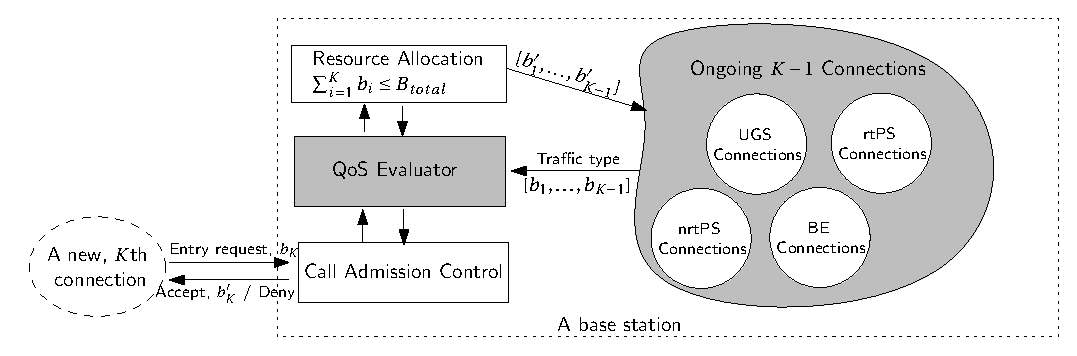
\includegraphics[width=0.95\textwidth]{cacop_qos_model_system.eps}
\caption{ 呼叫接纳控制的系统模型} \label{fig_system_model_cac}
\end{figure*}
%%%%%%
%QoS Metric
\subsection{QoS水平映射模型与带宽资源分配}
\esubsection{QoS Level Mapping Model and Resource Allocation}
在以往的大多数文献中,也出现了一些关于接纳控制方面的QoS研究工作。
他们对用户或系统的QoS评价指标一般从网络底层,如物理层或MAC层,直接获得。
譬如,带宽资源的利用率、掉话率或呼叫中断概率等等。
很少有从应用层QoS来研究呼叫接纳控制的。
实际上,对于用户从应用层感受到的QoS与底层网络QoS参数是区别的。
如果一个通信网络是以用户服务质量满意程度为设计原则的话,那么
对于业务连接的QoS评价也应该最好从应用层来评价。
但是,由于目前的通信网络是基于分层结构原则来设计的,上层如果需要传递给下层新的信息,就要大量修改或重新制定分层设计中的协议。
这样的改进对目前通信网络的结构冲击太大,需要对目前的通信网络进行大规模的改造,网络的实际布署困难很大。
因此,
我们提出可以通过一个预先构造好的QoS的映射模型,利用底层当前所能获得的参数信息将上层QoS参数估计出来。
这样就可以最大程度地兼容现有的通信网络。
对于业务连接而言,最重要的链路层网络参数就是它们所分配到的带宽资源 ~$\mathbf{b}$~。
如果通常这样一个简单的参数来估计用户的服务质量水平呢? 
下面,我们结合具体的业务类型实例,对连接所分配到的带宽资源与各项业务QoS之间的映射关系做详细的分析。

\begin{enumerate}[(1)]
    \item UGS业务与QoS评价:
        话音业务是UGS业务中最典型且最普遍的一种。
        而ITU提出的E模型(E-Model)提供了一种可以客观评价话音传输服务质量的方法 \cite{ITU:G107}。
        此模型通过提取网络参数(如延时或丢包)定义了对话音评估的分析模型。
        E模型可以使用R因子(R-factor)来评价话音质量。一般,R因子的值域在~$0$~到~$100$~之间。
        ~$0$~表示话音质量最差;~$100$~表示话音质量最好。在有些文献中,R因子会简化为另一个常用的评价指标,MOS(Mean Opinion Score)。
        MOS用~$1$~到~$5$~来评价话音质量。~$1$~表示最差的质量,~$5$~表示最好的质量\cite{NK:IEICE:2005}。

        R因子的值可通过\eqref{eqn:chap_cacop:FactorR}计算得到:
\begin{equation}
\label{eqn:chap_cacop:FactorR}
R = R_0 − I_s − I_d − I_e + A 
\end{equation}
其中,~$R_0$~ 表示基本的信噪比SNR。
~$I_s$~ 表示对于话音信号而言的损失之和。
~$I_d$~ 表示延时对通信的损害。
~$I_e$~ 表示由于低码率的编码方式对话音质量的影响。
~$A$~ 是一个优势因子(advantage factor),表示用户的容忍度。
为了计算方便,\eqref{eqn:chap_cacop:FactorR} 可以改写为经验\eqref{eqn:chap_cacop:FactorR_simple}
\begin{equation}
R = 93. 4 - I_d ( T_a ) -I_e ( codec, loss )
\label{eqn:chap_cacop:FactorR_simple}
\end{equation}
其中,~$I_d$~是一个单程延时函数。
%(在我们例子中,我们假设资源是以Kbps的单位进行分配的,同时分配的延时较小可以被忽略。)
~$I_e$~ 代表编码器的类型及丢包情况。
通过E模型计算器可得到不同的丢包状况下的话音质量R因子的值\cite{ITU:EModel:Caculator}。 
结果如表\ref{tb:R_factor}所示。
从表中的结果数据可以看出,话音业务对带宽资源极为敏感而且对丢包容忍度较低。
根据ITU提供的参考标准,R因子如果小于~$50$~则表明话音质量很差,用户很不满意。

\begin{table}[tb]
%\caption{R-Factor vs. Packet Loss} \label{tb:R_factor}
\setlength{\abovecaptionskip}{2pt}
\setlength{\belowcaptionskip}{8pt}
\caption{R因子与丢包率} \label{tb:R_factor}
\begin{center}
\wuhao
\begin{tabularx}{0.99\textwidth}{lXXXXXXXX}
%\begin{tabularx}{0.5\textwidth}{lp{9mm}}
\toprule 
丢包率(\%): & 0& 0.1& 0.3& 0.5& 0.7& 0.9& 1& 2\\
R-因子: &93.2& 84.6& 71.3& 61.5& 54.1& 48.2& 45.2& 29.9\\ 
\bottomrule
\end{tabularx}
\end{center}
\end{table}

因此,UGS业务的服务质量评估公式可以定义为,如\eqref{eqn:chap_cacop:metric_voice}所示。
\begin{equation}
\label{eqn:chap_cacop:metric_voice}
\alpha^{UGS}=
\begin{cases}
1 & \text{if $b=B$,}\\
0 &\text{others}
\end{cases}
\end{equation}
其中,~$\alpha^{UGS}$~ UGS业务流的服务质量QoS的值。
~$b$~是所分配到的带宽;
~$B$~表示此话音连接根据业务需要,申请的带宽资源数量。
为了表示简洁,
我们改写为Delta函数的形式,
\eqref{eqn:chap_cacop:Dirac_UGS}所示。
%
\begin{equation}
\label{eqn:chap_cacop:Dirac_UGS}
\alpha^{UGS}= \delta_{b}(B) = 
\begin{cases}
1 & \text{if $b= B$,}\\
0 &\text{others}
\end{cases}
\end{equation}

\item rtPS业务与QoS评价: 
rtPS应用中最典型的是视频应用。
在视频传输或编码研究中,峰值信噪比(peak signal-to-noise ratio,PSNR)是最常见的视频质量评价方法。
它采用的方法是将原始图像~$I$~与受损的重建图像~$K$~之间做逐像素的比较,
如\eqref{eqn:chap_cacop:psnr}所示。 
%
\begin{align}
\label{eqn:chap_cacop:psnr}
& PSNR = 10 \cdot \log_{10} \left( \frac{MAX_I^2}{MSE} \right)
\end{align}
其中,~$MAX_I$~ 是单个像素值域中的最大值。
如果每个像素点用~$8$~个比特表示,那么这个值就是~$255$~。
更一般的情况,如果每个像素采用~$z$~个比特表示,那么 ~$MAX_I$~就为 ~$2^z - 1$~。
分母部分是均方误差(mean squared error,MSE),表示原始图像~$I$~与解码重构图像~$K$~之间差。
它的定义为\eqref{eqn:chap_cacop:mse}。
%%%%%%
\begin{align}
\label{eqn:chap_cacop:mse}
MSE = \frac{1}{MN} \sum_{i=0}^{M-1}\sum_{j=0}^{N-1} \left[I(i,j) - K(i,j)\right]^2 
\end{align}
尽管PSNR在视频编码和解码研究领域广泛使用,但是它却不能直接在接纳控制单元中使用。
原因有两方面。一方面是,如果要想得到视频帧的PSNR的值,就要对压缩视频解码并恢复为YUV的图像帧。
这就意味着在MAC层中要嵌入视频解码单元。这一要求不太现实。
另一方面,PSNR的计算要有参考帧的图像。它是指压缩前的原始视频图像(Raw Picture)。
在一个通信网络中,这些数据对于接纳控制单元而言是不可能得到的。
而在数据链路层或MAC层所能得到的最重要的两个基本信息就是最终的带宽分配的情况~$b$~,以及业务连接对带宽需求的申请情况~$B$~。

最简单的方案是,可以类比网络吞吐量的定义,将~$\frac{b}{B}$~当做是评估视频连接的QoS。不幸的是,视频质量与比值~$\frac{b}{B}$~并不是简单的线性关系
 \cite{He1013856}。
所以,要寻找别的替代方案。这个替代方案要能够反应出服务质量与视频质量PSNR的关系,又能在数据链路或MAC层中方便地实现。
我们发现,率失真优化(rate distortion optimization,RDO)思想可以引入到我们的问题中来。
率失真优化是一种研究码率与压缩视频质量关系的方法
\cite{He1013856}\cite{E-H-Yang.TIP.2007} \cite{J-Y-Liu.ICIP.2009} 。
这种方法的目的是要建立视频的失真(损失)与所分配的码率之间的关系模型。
通过考察这个模型来对编码的码率做出指导。
从资源分配的角度看,视频质量与带宽分配之间也存在着类似的紧密联系。
为了能够找到一个合适的模型来描述视频质量与带宽分配之间的关系,我们尝试构造并比较了一些典型的拟合模型,对一些标准视频序列做了大量测试,详见附录1。 测试的结果比较类似。 例如,表\ref{tb:chap_cacop:fit_functions}就是结果之一。
\begin{table}[tb]
\caption{拟合模型与结果(以Foreman为例)} 
%\caption{Fitting Model Types} 
\label{tb:chap_cacop:fit_functions}
\centering
\wuhao
\begin{tabularx}{0.99\linewidth}{p{.1\textwidth}p{.4\textwidth}p{.2\textwidth}p{.2\textwidth}}
\toprule
ID& $f(x)$ & SSE & Adjusted R-square\\
\midrule
1&$ae^{bx}$ & 594.8 &0.4233\\
2&$p_1 x + p_2$ & 505.7 & 0.5096\\
3&$a_1e^{-((x-b1)/c1)^2}$&339.1&0.6243\\
4&$a_0 + a_1\cos(xw) + b_1\sin(xw)$&217.5&0.7317\\
5&$p_1x^2 + p_2x + p_3$ &207.5 & 0.7701\\
6&$p_1x^3 + p_2x^2 + p_3x + p_4$&62.04&0.9465\\
7&$a(1-e^{ \rho \frac{x}{\max(x)}})$ &19.83 & 0.9808\\
8&$p_1x^4 + p_2x^3 + p_3x^2 + p_4x + p_5$&14.93 &0.9871\\
\bottomrule
\end{tabularx}
\end{table}
表中的数据显示了不同拟合函数模型下,对视频测试序列“Foreman”的拟合结果。
从表中的结果可以看到,函数模型~$7$~和~$8$~性能明显优于其它模型。
对于不同的视频,模型~$7$~和~$8$~各有优劣。
比如Foreman,如果单从数学的拟合效果(Sum of Squares Due to Error(SSE) 和Adjusted R-square)来考虑,模型~$8$~ (~$p_1x^4 + p_2x^3 + p_3x^2 + p_4x + p_5$~)会更准确。
但是,此处我们统一选择模型 ~$7$~,~$a(1-e^{ \rho \frac{x}{\max(x)}})$~。 
选择它原因有三个:
一是,多项式模型使用了较多的系数来描述视频的特性。
而指数模型只有一个系数~$\rho$~来描述业务的特性。从模型的简洁程度来看,
指数模型更简单。
二是,指数模型有时尽管不如多项式模型~$8$~,但是它远优于其它的函数模型。
同时,它与最好多项式模型差距不大。
三是,指数模型可以涵盖其它类型的业务。
这样我们可以用统一的模型来表达多种业务的服务质量。
在接下来的内容中,我们将会解释这一点。

为了能兼容其它的业务,这里我们将指数模型进行归一化的处理,如
\eqref{eqn:chap_cacop:qos_level_users}所示。
\begin{equation}
\alpha^{rtPS} = \frac{PSNR_b}{PSNR_B} \approx \frac{1- e^{-\rho \frac{b}{B} }}{1-e^{-\rho}}, \rho > 0
\label{eqn:chap_cacop:qos_level_users}
\end{equation}
其中,
~$\alpha^{rtPS}$~ 表示归一化后的视频流或rtPS数据流的服务质量QoS。
~$PSNR_b$~ 和 ~$PSNR_B$~ 分别表示编码的码率为~$b$~ 和 ~$B$~的视频质量。
~$\rho$~ 代表 rtPS连接的数据流特征值。
每一个rtPS流都会有自己的特征值~$\rho$~。假定它在传输之前可以在编码器编码的过程中确定下来。
~$e^{-\rho \frac{b}{B}}$~部分表示失真。
~$1- e^{-\rho \frac{b}{B}}$~表示连接的QoS值。
分母~$1-e^{-\rho}$~是用来做归一化处理而引入的。
~$b$~ 表示当前连接所分配到的带宽数量,通常要求它大于它的最低带宽要求~$B_{\min}$~。
~$B$~表示当前连接需求的带宽数量。
为了进一步验证此模型有效,我们对不同标准视频序列按不同码率编码,结果如图 \ref{fig:chap_cacop:qos_rate_cac}所示。
图中的各项参数也是归一化后的。
为了便于比较,我们在结果图中增画一条~$\rho=4$~的曲线。
从图中各条曲线可以看到,所提出的以带宽参数值~$b,B$~及业务特征值~$\rho$~为基础的服务质量评估的模型可以用做rtPS或视频连接的服务质量的估计。
\begin{figure}[tb]
\begin{center}
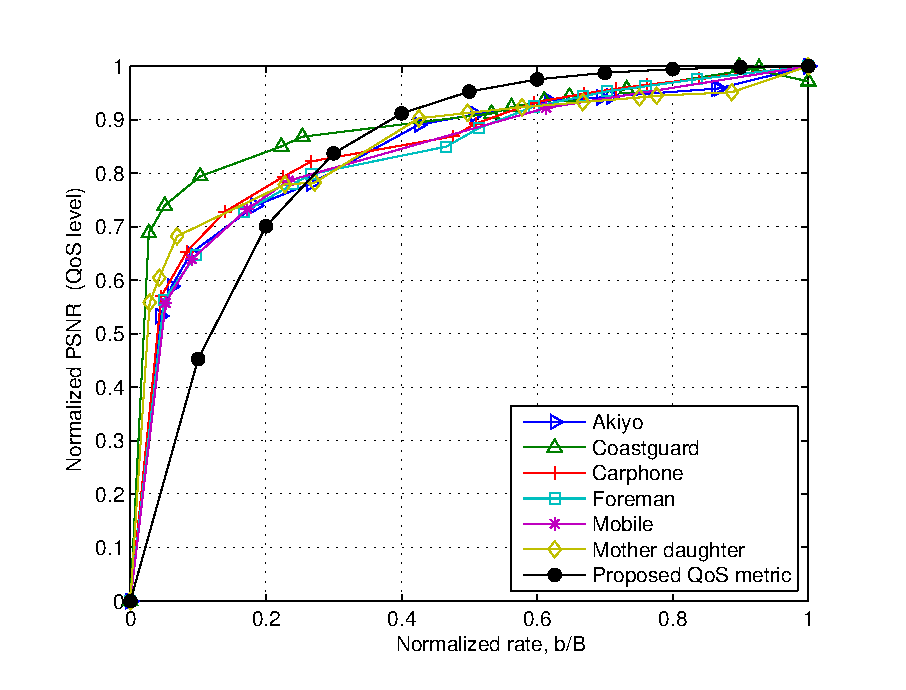
\includegraphics[width=0.75\textwidth] {cacop_qos_rate_cac.eps}
\end{center}
\caption{视频连接PSNR与码率的关系} 
\label{fig:chap_cacop:qos_rate_cac}
\end{figure}

\item 其它类型业务与QoS评价:
对于BE类型的业务,网页浏览HTTP应用或文件传输FTP应用是典型的例子。
HTTP(Hypertext Transfer Protocol)是互联网数据传输中最重要的应用层协议之一\cite{Fielding_1999}。 
由于其简捷、快速的方式特点,适用于分布式超媒体信息系统。
FTP是用于在网络上进行文件传输的一套标准协议。它也属于网络协议组的应用层。用于Internet上的控制文件的双向传输。
同时,它也是一个应用程序(Application)。用户可以通过它把自己的计算机与运行FTP协议的服务器相连,访问和下载服务器上的程序和数据 \cite{Postel_Reynolds_1985}。
这两类业务应用的共同点是用户对服务质量的要求取决于在发送端发送数据的总量与接收端已接收数据量的多少。
所以,我们把这类应用的服务质量简单地定义为\eqref{eqn:chap_cacop:BE_metric} 。
%
\begin{equation}
\label{eqn:chap_cacop:BE_metric}
\alpha^{others} = \frac{b}{B}
\end{equation}
%
其中,~$b$~是分配得到的带宽资源,~$B$~是对于BE类应用而言所需的带宽资源。
它们的比值就可以表示这类应用连接的服务质量水平。
为了简单起见,对于业务nrtPS,假定此类业务特征与BE的类型类似,也用 \eqref{eqn:chap_cacop:BE_metric} 表示。
\end{enumerate}

综上所述,因为各类业务的服务质量计算公式差别不大,下面将它们总结一下。
我们注意到\eqref{eqn:chap_cacop:qos_level_users}在业务特征值~$\rho$~趋向于$0$时存在极限,如\eqref{eqn:BE_limit}所示。
而且,它恰好是BE业务的服务质量计算公式。 所以,可以假设这类业务的特征值$\rho$很小。
%
\begin{equation}
\label{eqn:BE_limit}
\lim\limits_{\rho \to 0 } \frac{1- e^{-\rho \frac{b}{B} }}{1-e^{-\rho}} = \frac{b}{B}
\end{equation}

所以我们将\eqref{eqn:chap_cacop:BE_metric}改写为\eqref{eqn:chap_cacop:BE_metric_2}。
%
\begin{equation}
\label{eqn:chap_cacop:BE_metric_2}
\alpha^{others} = \frac{b}{B} = \frac{1- e^{-\rho \frac{b}{B} }}{1-e^{-\rho}} \quad \text{if} \quad \rho \to 0
\end{equation}
%

最后,将各种业务类型的服务质量评估公式整理后,可得\eqref{eqn:chap_cacop:alltype_metric}。
%
\begin{equation}
\alpha = 
\begin{cases}
\delta_{b}(B), &\text{for UGS} \\
\frac{1- e^{-\rho \frac{b}{B} }}{1-e^{-\rho}}, \rho > 0& \text{for rtPS }\\
\frac{1- e^{-\rho \frac{b}{B} }}{1-e^{-\rho}}, \rho>0, \rho \to 0, &\text{for BE, nrtPS}\\
\end{cases}
\label{eqn:chap_cacop:alltype_metric}
\end{equation}

\section{基于QoS映射模型的资源分配优化与接纳控制算法}
\esection{Optimum of Resource Allocation and CAC alogorithm with QoS Level Mapping Model}
\subsection{资源分配的优化}
\esubsection{Optimum of Resource Allocation}
接纳控制的本质是为了保证各个连接良好的通信服务质量,防止新连接占用资源后对在线连接产生负面的影响。
一个好的接纳控制方法应该在充分利用资源的前提下,保证用户的服务质量最大化。
因此,可以将这个问题归结为一个如下的优化问题。
假设在系统中有~$M$~个 UGS连接,~$N$~个 rtPS 连接和 ~$Q$~个其它类型的连接。而且,这些连接之间是彼此无关的。
那么,所有连接的QoS值之和可以表示为基站的整体效用,如\eqref{eqn:chap_cacop:bs_qos} 所示。
\begin{align}
U_{BS} &= \displaystyle \sum_{i=1}^K \alpha_i \nonumber \\
&= \sum_{i=1}^M\alpha_i^{UGS} + \sum_{i=1}^N\alpha_i^{rtPS} + \sum_{i=1}^Q\alpha_i^{others} \nonumber \\
&=\displaystyle M^\prime + \sum_{i=1}^N \left( \frac{1- e^{-\rho_i^r
\frac{b_i}{B_i} }}{1-e^{-\rho_i^r}} \right)
 + \sum_{i=1}^Q \left( \frac{1- e^{-\rho_i^o
\frac{b_i}{B_i} }}{1-e^{-\rho_i^o}} \right),
\label{eqn:chap_cacop:bs_qos}
\end{align}
其中,~$M^\prime(\le M)$~ 表示~$M^\prime$~ 个UGS连接分配到了所需的带宽资源。
~$\rho_i^r$~ 是第~$i$~个rtPS连接的数据流特征。 
~$\rho_i^o$~ 表示其它类型(others)的连接特征。此处,我们假定这个值~$\rho_i^o$~很小。
因为~$\rho_i^r$~ 和~$\rho_i^o$~都表示数据流的特点,只是值的大小不同。所以,可以用符号~$\rho_i$~来统一表示~$\rho_i^r$~ 和~$\rho_i^o$~。
~$U_{BS}$~ 表示基站在给~$K$~个连接提供服务所能获得的整体效用。
如果~$U_{BS}$~有最大值, 那么一定存在一个资源分配的优化解
~$\mathbf{b}$~ 。
在后面,我们会把这个解做为接纳控制的判决条件。
因此,这个优化问题可为如下形式。
\begin{align}
\mathbf{b}^* &= \arg \max \left\{ U_{BS}(\mathbf{b}) \big| \mathbf{b} = [b_1, b_2, \dots, b_K] \right\} \label{eqn_u_bs_qos}\\
&\text{subject to:}\nonumber\\
&\displaystyle\sum_{i=1}^{K}b_i + B_{ava}= B_{total} \nonumber
\end{align}
其中, ~$\mathbf{b}^*$~ 是资源分配的优化解。
~$B_{total}$~ 是系统所能提供的全部带宽。
~$ B_{ava} $~是剩余的带宽资源。

因为接纳控制通常是在业务负载大的情况下产生作用,所以为了简单起见,
我们假设剩余资源为零。同时,因为UGS类型的连接对带宽的要求严格,所以这些连接必须按照申请的数量分配。
我们则将上面的优化问题改写为 \eqref{eqn:chap_cacop:final_opt_qos}。
\begin{align}{}
\label{eqn:chap_cacop:final_opt_qos}
\mathbf{b}^* &= \arg \max \left\{ U_{BS}(\mathbf{b}) \big| \mathbf{b} = [B_1, B_2, \dots,B_M,\right.
 \left. b_{M+1}, \ldots, b_K] \right\} \\
&\text{subject to:}\notag \\
&\sum_{i=1}^M B_i + \sum_{i=M+1}^{K}b_i= B_{total} \notag
\end{align}

下面来解这个优化问题。
先要证明这个优化问题存在解。
为了方便书写,引入一个新的变量~$x$~来表示~$\frac{b}{B}$~。
\begin{equation*}
\begin{split}
x_i = \frac{b_i}{B_i} , i \in [M+1, K].
\end{split}
\end{equation*}
然后,引入拉格朗日乘子~$\lambda$~,写出所需的拉格朗日方程,如
\eqref{eqn:chap_cacop:lagrange_defination}所示。
%%%
\begin{align}
&\displaystyle F(x_{M+1}, x_{M+2}, \dots, x_K, \lambda)= \sum^{M+N}_{i=M+1}
\left( \frac{1-e^{-\rho_i x_i}}{1-e^{-\rho_i}} \right) \nonumber \\
& \qquad \displaystyle +\sum_{i=M+N+1}^K\left( \frac{1-e^{-\rho_i x_i}}{1-e^{-\rho_i}} \right) 
 + \lambda
\left(B_{total} - \sum_{i=1}^M B_i -\sum^K_{i=M+1} x_i B_i \right).
\label{eqn:chap_cacop:lagrange_defination}
\end{align}
%%%
而后,对上面方程求两阶导数~$\frac{\partial ^2F}{\partial x_i \partial x_j}$~得Hermitian矩阵~${M}$~。
%%%
\begin{eqnarray*}
{M} = & 
\left[
\begin{array}{cccc}
\frac{\partial ^2F}{\partial x_{M+1} ^2} &\frac{\partial ^2F}{\partial x_{M+1} \partial x_{M+2}} & \dotsi & \frac{\partial ^2F}{\partial x_{M+1} \partial x_K} \\
\frac{\partial ^2F}{\partial x_{M+2} \partial x_{M+1}}& \frac{\partial ^2F}{\partial x_{M+2} ^2}& \dotsi & \frac{\partial ^2F}{\partial x_{M+2} \partial x_K}\\
\vdots & \vdots & \ddots & \vdots \\

\frac{\partial ^2F}{\partial x_{K} \partial x_{M+1} } &\frac{\partial ^2F}{\partial x_{K} \partial x_{M+2}} & \dotsi&\frac{\partial ^2F}{\partial x_K ^2}\\
\end{array}
\right] \\
=&
\left[
\begin{array}{cccc}
\frac{-\rho_{M+1}^2 e^{-\rho_{M+1} x_{M+1}}}{(1-e^{-\rho_{M+1}})} & & & \text{{\huge{0}}}\\
&&\ddots\\
\text{{\huge{0}}} &&& \frac{-\rho_{K}^2 e^{-\rho_{K} x_{K}}}{(1-e^{-\rho_{K}})}\\
\end{array}
\right] 
\end{eqnarray*}
很明显,如果~$\rho >0$~ ,那么~$1-e^{-\rho} >0$~。
矩阵~${M}$~是负定的(negative-definite)。
因此对于BS的效用~$U_{BS}$~来说,如果有驻点存在,则是局部极大值点。
下面来求一阶导数为零时的驻点。
首先让对拉格朗日函数求一阶导数,并置为零,
~$dF = 0$~,则有下面一系列式子。
%%%
\begin{align} 
\begin{cases}
\frac{\partial F}{\partial x_{M+1}} =
\frac{\rho_{M+1} e^{-\rho_{M+1} x_{M+1}}}{(1-e^{-\rho_{M+1}})} - \lambda B_{M+1} = 0 \\
\frac{\partial F}{\partial x_{M+2}} =
\frac{\rho_{M+2} e^{-\rho_{M+2} x_{M+2}}}{(1-e^{-\rho_{M+2}})} - \lambda B_{M+2} = 0 \\
\qquad \vdots \qquad \vdots \qquad \vdots \\
\frac{\partial F}{\partial x_K} =
\frac{\rho_K e^{-\rho_K x_K}}{(1-e^{-\rho_K})} - \lambda B_K = 0 \\
\frac{\partial F}{\partial \lambda} = B_{total} - \sum_{i=1}^M B_i -
\sum^K_{i=1}x_iB_i = 0 
\end{cases}
\label{eqn:chap_cacop:derivate}
\end{align}
%%%


根据\eqref{eqn:chap_cacop:derivate},我们有
%%%
\begin{equation*}
\begin{split}
&\frac{\partial F}{\partial x_i} = \frac{\rho_i e^{-\rho_i
x_i}}{(1-e^{-\rho_i})} - \lambda B_i = 0\\
\implies &\rho_i e^{-\rho_i x_i} =\lambda B_i(1-e^{-\rho_i})\\
\implies &\ln\rho - \rho x_i = \ln [\lambda B_i (1-e^{-\rho_i})]\\
\implies &x_i = \frac{1}{\rho_i} \ln \left[ \frac{\rho_i}{\lambda B_i(1-e^{-\rho_i})} \right] \\
\end{split}
\end{equation*}
%%

再将 ~$x_i$~ 代入\eqref{eqn:chap_cacop:derivate}中的最后一个,则又有
%%%
%
\begin{equation}
\begin{split}
&B_{total} -\sum_{i=1}^MB_i = \sum_{i=M+1}^K x_i B_i \\
&= \sum_{i=M+1}^K \frac{B_i}{\rho_i} \ln \left[ \frac{\rho_i}{\lambda B_i(1-e^{-\rho_i})} \right] \\
%&= \sum^K_{i={M+1}}\left[- \frac{1}{\rho_i}\ln \lambda - \frac{1}{\rho_i}
%\ln (B_i) - \frac{1}{\rho_i} \ln (1-e^{-\rho_i}) + \frac{1}{\rho_i}
%\ln
%\rho_i \right] B_i\\
%&= \sum^K_{i={M+1}}\left[- \frac{B_i}{\rho_i} \ln \lambda -
%\frac{B_i}{\rho_i} \ln (B_i) - \frac{B_i}{\rho_i} \ln (1-e^{-\rho_i})
%+ \frac{B_i}{\rho_i} \ln
%\rho_i \right]\\
%&= -{\ln \lambda}\sum^K_{i={M+1}} \frac{B_i}{\rho_i} 
%- \sum^K_{i={M+1}} \frac{B_i \ln (B_i)}{\rho_i} 
%- \sum_{i={M+1}}^K \frac{B_i\ln(1-e^{-\rho_i})}{\rho_i} \\ 
%& \hspace{5mm}+ \sum^K_{i={M+1}} \frac{ B_i\ln \rho_i} {\rho_i} \\
\end{split}
\label{eqn_find_mu}
\end{equation}

%%%
根据公式 (\ref{eqn_find_mu}), 我们可以解出~$\lambda$~.
%%%
\begin{equation*}
\begin{split}
\lambda &= \exp \left( \frac{\sum_{i=M+1}^K \frac{B_i}{\rho_i} \ln \left[ \frac{\rho_i}{B_i(1-e^{-\rho_i})} \right]
}{\sum_{i=M+1}^K \frac{B_i}{\rho_i}} \right.
+ \left. \frac{ 
\sum_{i=1}^M B_i - B_{total}}{\sum_{i=M+1}^K \frac{B_i}{\rho_i}} \right)\\
\end{split}
\end{equation*}
%%%

然后,可以求得
%%%
%
\begin{equation}
\begin{split}
x_i & = \frac{1}{\rho_i} \ln \frac{\rho_i}{B_i(1-e^{-\rho_i})} \\
&-\frac{1}{\rho_i}\left( \frac{\sum_{j=M+1}^K \frac{B_j}{\rho_j} \ln \left[\frac{\rho_j}{B_j(1-e^{-\rho_j})}\right] 
}{\sum_{j=M+1}^K \frac{B_j}{\rho_j}} \right)
-\frac{1}{\rho_i}\left( \frac{ 
\sum_{j=1}^M B_j - B_{total}}{\sum_{j=M+1}^K \frac{B_j}{\rho_i}} \right) \\
\end{split}
\end{equation}
%
%%%

最后,整理可得带宽分配的解。
%
\begin{equation}
\begin{split}
\mathbf{b^*}& = [b^*_{M+1}, \cdots, b^*_{K}]\\
b_i^* & = x_iB_i = \frac{B_i}{\rho_i} \ln \frac{\rho_i}{B_i(1-e^{-\rho_i})} \\
&-\frac{B_i}{\rho_i}\left( \frac{\sum_{j=M+1}^K \frac{B_j}{\rho_j} \ln \left[\frac{\rho_j}{B_j(1-e^{-\rho_j})}\right] 
}{\sum_{j=M+1}^K \frac{B_j}{\rho_j}} \right)
 -\frac{B_i}{\rho_j}\left( \frac{ 
\sum_{j=1}^M B_j - B_{total}}{\sum_{j=M+1}^K \frac{B_j}{\rho_i}} \right),  \\ 
 & \hspace{75mm} i \in [M+1, \cdots, K] \\
\end{split}
\label{eqn:chap_cacop:b_i_bw}
\end{equation}

所以,可知存在一个驻点。

综上所述,由二阶条件的负定及一阶条件及上面的驻点,可知这个资源分配方案$\mathbf{b^*}$是使基站系统的整体效用取得最大值的解。
%
\subsection{接纳控制算法}
\esubsection{Proposed CAC algorithm}
\label{sec_alg}

\begin{algorithm}[htbp]
\SetAlgoLined
% assume ~$B_{ava}=0$~\;
等待一个新的连接进入请求;假定此时系统中有~$K-1$~连接正在进行通信\;
新连接~$K$~申请进入。其中,申请资源数量为$B_K$\;
\eIf {~$B_K<= B_{ava}$~}{
允许连接~$K$~进入系统,被分配带宽~$B_K$~\;
}{
根据资源分配\eqref{eqn:chap_cacop:b_i_bw}计算~$\bf b^*$~\;
检查在线连接的资源分配计算值~\;
\If{~$b_i^* < B_i^{\min} $~}{
连接~$i$~被系统列入本次的保护范围~\;
~$B_{total} = B_{total} - b_i^{old}$~\;
参加优化计算的连接总数减一 \;
{\bf{go to 6}}\;
}
检查新连接~$K$~的资源分配计算值~\;
\eIf{~$b_K< B_K^{min}$~}{
拒绝新连接~$K$~的请求\;
{\bf{go to 1}}\;
}{
允许新连接~$K$~进入系统\;
\For{~$i=1$~ \KwTo ~$K-1$~}{
被保护的连接继续保持已经得到的资源数量不变\;
对于其它的连接按计算后的优化资源分配方案~$b_i$~执行\;
}
分配资源~$b_K^*$~ 给新连接~$K$~\;
}
}
{\bf{go to 1}}\;
\caption{提出的接纳控制算法 (NQoSCAC)} \label{alg:chap_cacop:agr_cac}
\end{algorithm}


根据上一节所得到的带宽分配方案,我们提出一个接纳控制算法,称之为NQoSCAC, (Normalized QoS CAC )。
在此算法中,涉及到两个常见的假设。 一是假设分配到资源数量应该大于业务所需的最小数量,即
~$b_i^* \ge B_i^{\min}$~. 
这个最小值与业务的类型相关。不同业务均有所不同。
例如,对于话音应用来说,它所需的带宽的最小值就被设置为它申请值。
对于视频这样的rtPS应用,一般~$b_i\ge B_i^{\min}$~。
对于新用户~$K$~而言,
如果~$b_K^*$~ 小于所需的资源的最小值~$B_K^{\min}$~,意味着系统会拒绝这个连接进入。
因为如果按这样的资源量分配给连接~$K$~,服务质量会很差,用户肯定不满意。
二是,
在我们提出的算法中,使用了优级的概念。我们假设在线连接的优先级要比新连接的优先级要高。这样的假定会使得在线用户的通信不会被中断。

因为引入了上述的两个假设,所以在我们的算法中,会在带宽分配的过程中出现迭代。
比如,如果一个在线的连接由资源分配 \eqref{eqn:chap_cacop:b_i_bw}计算所得的资源数量小于它的最小资源需求数量,我们认为这个连接应该受到保护。
接纳算法会将取消此次计算过程,将此连接和它占用的资源排除在外,
然后重新启动一轮的带宽计算过程。
直到不再出现在线连接所分配的资源会小于它最低要求。
对于连接~$K$~来说,如果最后的结果大于其最低资源要求,则允许其进入系统;否则,这个连接会被系统阻塞(blocked)。


当一个新连接提出进入系统的申请时,接纳控制单元启动CAC过程。
如果当前的空闲资源大于新连接~$K$~所需的资源数量,
那么新连接会被允许进入系统接受服务,并分配给资源~$B_K$~。
否则,系统进入优化资源分配的计算过程。
在一个空闲资源缺乏且系统负载大的情况下,一个新连接被系统接纳需要满足两个条件:
一是对于新连接~$K$~来说,优化的资源分配值~$b_K$~要大于最低资源需求~$b_K^{\min}$~。
另一个是对于其它在线的连接所分配到是优化资源值~$b_i$~也要大于各自的最低资源需求。
正是因此原因,算法会尽可能将基站系统的整体效用保持在较高的水平的基础;同时,也兼顾了单个连接的需求。
算法的详细流程如流程{\bf{ 算法 \ref{alg:chap_cacop:agr_cac}}} 所示。
其中,步骤7、8、9用来将那些需求保护的连接排除出分配方案中。
%%算法描述


\section{仿真实验与结果分析}
\esection{Simulation and Results}
\begin{figure*}[tb]
\centering
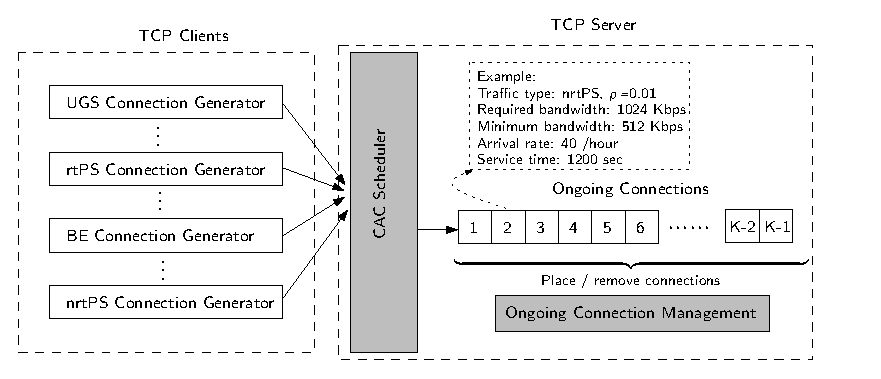
\includegraphics [scale=1.2] {cacop_simulator.eps}
\caption{系统仿真模型} 
\label{fig:chap_cacop:sim_cfg}
\end{figure*}
我们通过构造一个系统的仿真模型来评估所提出的算法。
这个仿真的模型如\figref{fig:chap_cacop:sim_cfg} 所示。
为了能够去除一些仿真中的随机因素,仿真脚本被运行多次来得到一个统计意义的结果。

\subsection{仿真模型}
\esubsection{Model of Simulation System}
我们根据本章第三小节介绍呼叫接纳控制模型,建立了这样一个仿真模型。
模型包括下面几个组成部分:
\begin{itemize}
\item 伪连接产生单元(Pseudo Connection Generators): 它能够按照泊松分布产生新的连接,就象在排队论中“顾客”。
    相邻的两个连接到达的时间间隔~$T$~来自于一个指数分布,用\eqref{eqn:chap_cacop:exp_model}定义。
%
\begin{equation}
\label{eqn:chap_cacop:exp_model}
F_T(t) = 1 - P_0(t) = 1 - e^{-\lambda t}
\end{equation}
%
\begin{table}[tb]
\caption{连接的业务类型} \label{tb:chap_cacop:sim_cfg}
\begin{center}
\wuhao
\begin{tabularx}{0.99\linewidth}{XXXXXp{2.5cm}}
\toprule
业务类型 &~$\rho$~ &所需的带宽 & 最小的带宽 &到达率 &接受服务时间 \\
%Type & &bandwidth & bandwidth & rate & time \\
&&(Kbps)& (Kbps) & (/hour) &(seconds) \\
\midrule
UGS& N/A &64 &64 & 100 &600\\
BE & 0.01&90 &64 &90 &700\\
rtPS &4& 128 &64 &80 &800\\
rtPS &5& 256 &128 &70 &900\\
BE &0.01& 384 &192 &60 &1000\\
nrtPS &0.01& 768 &384 &50 &1100\\
nrtPS &0.01& 1024 &512 &40 &1200\\
rtPS &6& 1512 &756 &40 &1200\\
rtPS &7& 1768 &884 &30 &1500\\
rtPS &8& 2048 &1024 &30 &1500\\
\bottomrule
\end{tabularx}
\end{center}
\end{table}
连接到达率根据不同业务类型及应用设定为每小时 ~$30 \text{ to } 100 $~。
每个连接都设置有最小带宽需求与业务类型特征值。
带宽需求数量在64Kbps到2Mbps之间。
并且,假设连接在系统内为停留时间(接受服务的时间)为一个均值为600到1500秒指数分布的随机变量。
表\ref{tb:chap_cacop:sim_cfg}详细地列出其中的各项参数。

\item 在线连接管理单元(Ongoing Connection Management): 当一个连接被系统接入后,它会被放入一个队列中进行管理。当它的服务时间结束时,管理单元会将它从队列中删除。

\item 呼叫接纳控制单元(Call Admission Control Scheduler): 此单元负责计算每一个连接应分配的资源数量,并分配总共~$B_{total}=75Mbps$~的带宽资源。 
\end{itemize}
作为对比算法,我们使用了两种常见的方法。
第一个标记为“Baseline”。这种方法在进行接纳判断时,只是根据剩余的空闲带宽能否满足新连接的要求。
如果空闲带宽足够,则接入;否则,则拒绝进入。
另外一种是由学者EL Kadi提出的资源保留算法。该算法在系统的总资源中保留一定比例专门针对新连接的接入\cite{EL-Kadi2002}。
%%%%%
\subsection{仿真结果}
\esubsection{Results and Analysis}
%
\begin{table}[htbp]
\caption{仿真结果汇总} \label{tb:chap_cacop:res_sim}
\begin{center}
\wuhao
\begin{tabularx}{0.99\textwidth}{XXXX}
\toprule
&Baseline &Elkadi &Proposed (NQoSCAC)\\
\midrule
阻塞率 (\%) &4.15 & 0 &0.82\\
资源利用率(\%) &86.70 &83.57 &88.42\\
系统连接容量 &137.55 &145.60 &144.01\\
连接的平均QoS &1.00 &0.94 &0.98\\
基站系统的效用 &137.55 &136.28 &141.19\\
\bottomrule
\end{tabularx}
\end{center}
\end{table}
表 \ref{tb:chap_cacop:res_sim} 汇总了三种方法的仿真统计结果。
在仿真过程中,我们除了考察传统的 CAC 性能指标,如新连接的阻塞率,资源利用率以及系统连接容量,而且还评估了本章所提出的QoS的测量值,以及基站系统的整体效用。
在三种方法中,我们所提出的算法在资源利用率及系统效用方面性能表现最好,
资源利用率分别比其它两个方法高~$2\%$~和~$4\%$~;系统整体效用值比其它两个方法高约4和5。
在阻塞率这一项,所提出的方法与基准方法“Baseline”相比较,阻塞率下降了五倍,从~$4.15\%$~ 降至为 ~$0.82\%$~。
此外,因为在ELKadi的资源预留方法中,资源对新连接总是优先使用的,所以这种方法会将新连接的阻塞率降为零。
而我们所提出的方法为~$0.82\%$~,与ELKadi方法比较接近。
从各项指标的整体来看,我们所提出的方法综合的性能较优。
%The baseline method maximizes the average QoS level of the ongoing connections, because it must block new connections in the heavy traffic load condition. 
%%%%%%%
%
\begin{figure}[htbp]
\centering
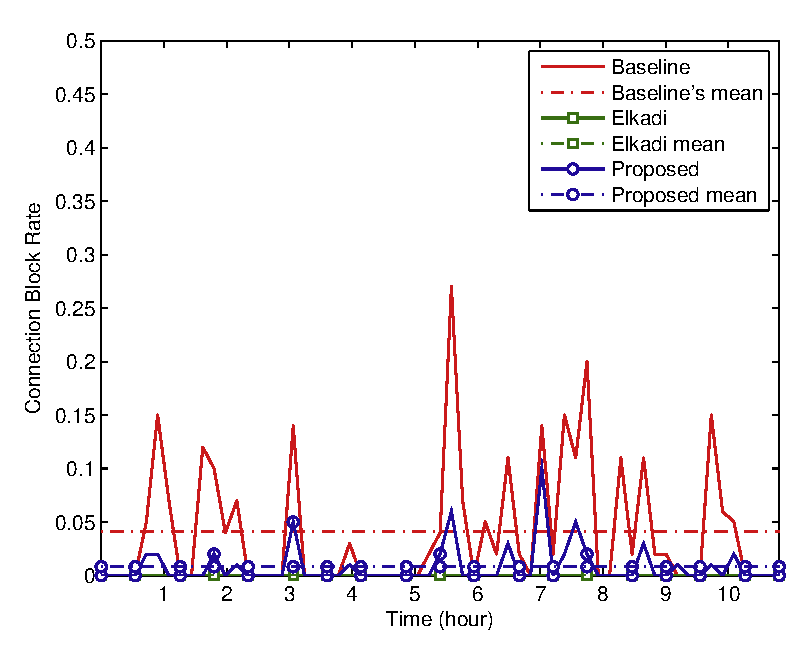
\includegraphics[width=0.65\textwidth] {cacop_block_rate.eps}
\caption{新连接的阻塞率} \label{fig:chap_cacop:clock_accept_block_drop}
\end{figure}

%%%%%%%
%
\begin{figure}[htbp]
\centering
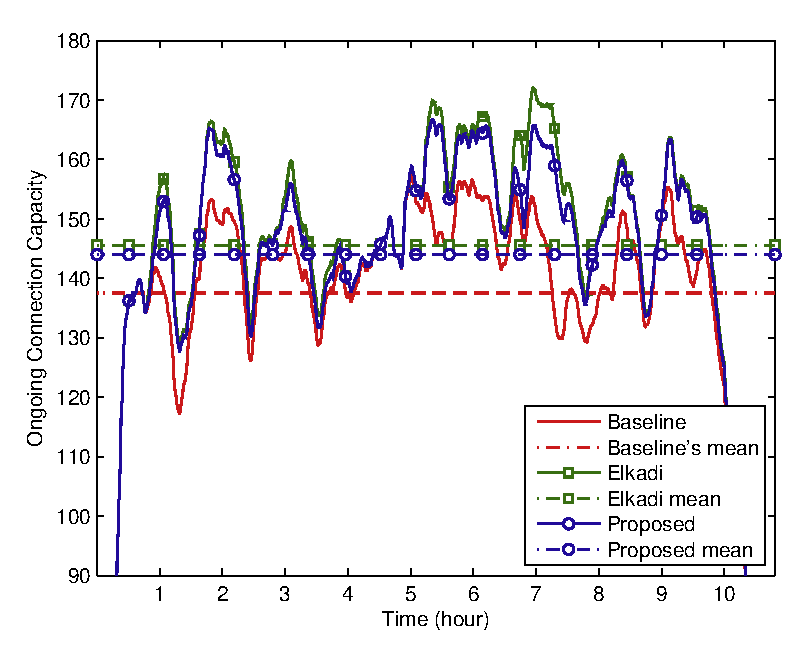
\includegraphics[width=0.65\textwidth] {cacop_conns_sum.eps}
\caption{系统的在线连接容量}\label{fig:chap_cacop:clock_onging_call_sum}
\end{figure}

%%%%%%%
% 
\begin{figure}[htbp]
\centering
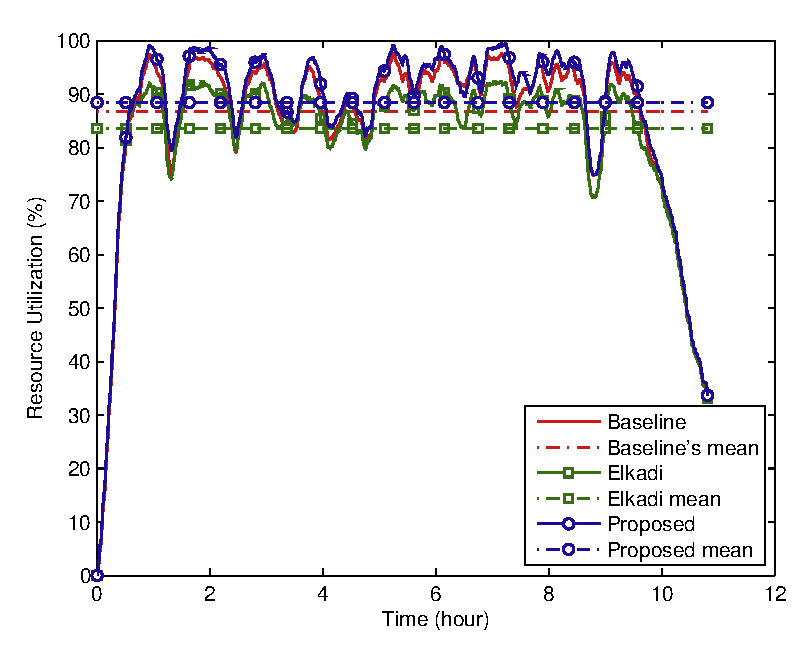
\includegraphics[width=0.65\textwidth]{cacop_bw_utilization.eps}
\caption{系统资源利用率}\label{fig:chap_cacop:clock_bs_availble_bw}
\end{figure}

%%%%%%%
%
\begin{figure}[htbp]
\centering
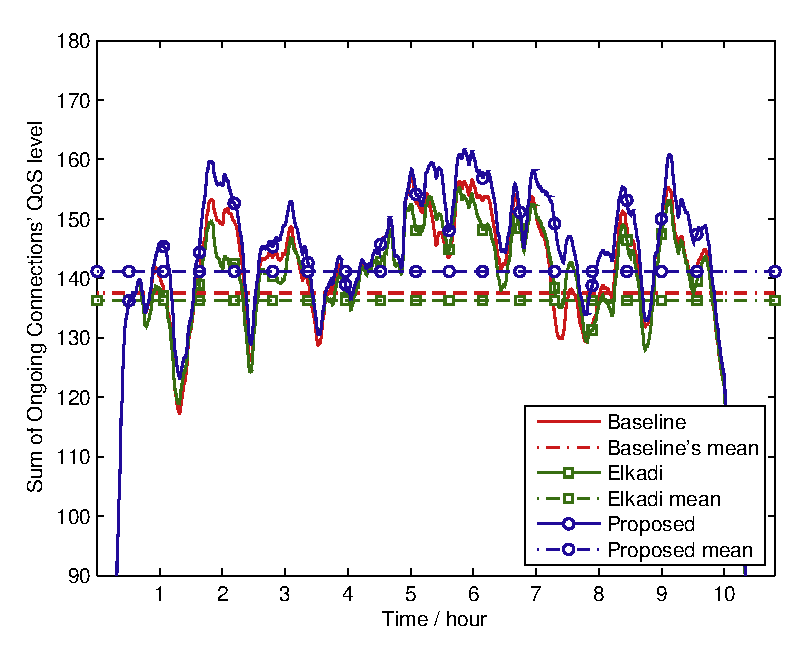
\includegraphics[width=0.65\textwidth] {cacop_qos_sum.eps}
\caption{基站系统效用}\label{fig:chap_cacop:clock_bs_qos_sum}
\end{figure}

%%%%%%%
% 
\begin{figure}[htbp]
\centering
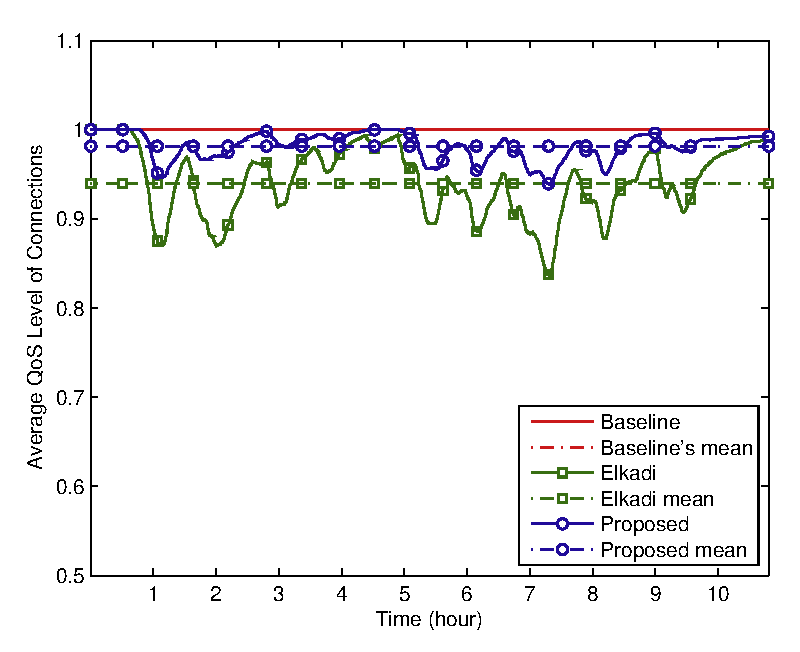
\includegraphics[width=0.65\textwidth] {cacop_avg_qos.eps}
\caption{连接平均QoS水平}\label{fig:chap_cacop:clock_avg_call_qos}
\end{figure}


%On contrast, the proposed method can increase by up to 6 \% bandwidth utilization by making the slight degradation of block rate. The performance of the QoS level of BS can achieve the best one among them to 141.4 while the average QoS level of connections is kept as 0.984, just to decrease by 0.16 in comparison with maximum value, one. 

另一方面,\figref{fig:chap_cacop:clock_accept_block_drop} 到 \figref{fig:chap_cacop:clock_avg_call_qos} 显示了各个性能指标在整个仿真过程中的实时情况。
这里的每一幅图中我们绘制了六条线。其中,水平的虚线是不同算法的性能指标的均值。

如\figref{fig:chap_cacop:clock_accept_block_drop}所示,采用我们的方法,新连接的阻塞率在整个仿真的过程中均保持着很低的水平。
同时,还可清楚地看到“Baseline”算法的阻塞率波动较大。
\figref{fig:chap_cacop:clock_onging_call_sum} 显示了在线连接的个数(系统容量),可以看出,ElKadi方法与本文所提算法曲线非常接近,且明显优于基准算法。
对于资源利用率,与其它二个算法相比较,ElKadi的性能最差。这也可以看出预留算法的缺陷。由于在高业务负载下,预留算法为了保证新连接能够及时的接入,使得一部分的资源未得到充分地利用,如 \figref{fig:chap_cacop:clock_bs_availble_bw}所示。
 
从用户的角度看,QoS水平曲线对于单个用户更有意义一些。
如\figref{fig:chap_cacop:clock_avg_call_qos}所示,
这些曲线表示的是在线用户的QoS水平和满意度。我们所提出的方法明显优于ElKadi的算法。同时,我们还可看出,基准算法的平均QoS水平总是最高的,始终维持在常量最大值~$1$~。基准算法通过牺牲新连接服务质量,使得在线用户服务质量得到了最大程度的保证。
从这些仿真结果,我们清楚地看到,在一个资源受限的系统中,系统性能指标之间是存在矛盾的。通常其中一个性能指标得到改善和提高的同时,会使得另外一个性能指标下降。譬如在线用户的QoS水平与新用户的阻塞率。总的来说,从仿真的结果来看,我们所提出的算法在平衡相互矛盾的系统指标方面,比其它两种方法要好。我们的算法兼顾了新用户与在线用户的利益,并进行了很好的平衡与折衷。

\section{本章小结}
\esection{Chapter Summary}
本章研究的是基于多媒体业务特征的呼叫接纳控制问题。
首先我们通过分析不同的多媒体业务特点,
建立一个网络底层资源分配参数与网络高层的业务QoS水平的映射机制,
实现不同业务用户或不同内容特点的连接的QoS统一标定与测量。 
并且,基于这个映射模型,提出了一个基于在线用户和与新用户利益兼顾呼叫接纳控制与资源分配的优化算法,
实现不同业务QoS以及系统资源的有效管理与分配。
该算法以系统整体服务质量效用为最大化目标,在高负荷下依据用户业务负载情况调整接纳与分配策略,可以让各项性能指标得到较好的平衡与折衷。
%
%%
%%


